\documentclass[12pt,letterpaper]{article}
\usepackage[margin=1in]{geometry}
\usepackage{graphicx}
\usepackage{subfig}
\usepackage{color}
\usepackage{enumerate}
\usepackage{mathtools}
%\usepackage{amsfonts}
%\usepackage{amssymb}
%\usepackage{MnSymbol}
\usepackage{amsmath}
\usepackage{amsthm}
\usepackage{commath}

% Common parenthetic remarks
\newcommand{\ie}[1]             {(\textit{i.e.} #1)}
\newcommand{\eg}[1]             {(\textit{e.g.} #1)}

\newcommand{\N}					{{\mathbb N}}
\newcommand{\Z}					{{\mathbb Z}}
\newcommand{\Q}					{{\mathbb Q}}
\newcommand{\R}					{{\mathbb R}}
\newcommand{\C}					{{\mathbb C}}
\newcommand{\F}					{{\mathbb F}}
\newcommand{\T}					{{\mathbb T}}

% Macro for defining space in integral between integrand and infinitesimal
\renewcommand{\d}{\,d}

\newcommand{\gradient}[1]       {\vec{\nabla}#1}

% Distinguish bars in code
\newcommand{\conj}[1]			{\overline{#1}}
\newcommand{\mean}[1]			{\overline{#1}}

% I like operator form rather than weird font
\renewcommand{\Re}[1]			{\operatorname{Re}\left(#1\right)}
\renewcommand{\Im}[1]			{\operatorname{Im}\left(#1\right)}

% Set complement
\newcommand{\stcomp}[1]		   	{{#1}^\mathsf{c}}
\newcommand{\closure}[1]		{\overline{#1}}

% Directional derivative
\newcommand{\dirderiv}[2]       {\vec{\nabla}#1\cdot \hat{#2}}  

\newcommand\supp                {\mathop{\rm supp}}
\newcommand\sign[1]             {\mathop{\rm sgn}\del{#1}}

\DeclarePairedDelimiter{\ceil}{\lceil}{\rceil}

\newcommand\unitvec[1]          {\vec{\hat{#1}}}
\renewcommand\vec[1]            {\mathbf{#1}}

\begin{document}
% No automatic indenting
\setlength{\parindent}{0pt}

\section{Introduction}
Unittest is configured such that
\begin{itemize}
\item{the coarsest level\footnote{AMReX uses 0-based level indexing whereas
FLASH uses 1-based indexing.  We adopt the FLASH convention here so that the coarsest
level is level 1.} has 2 blocks along both the X and Y
coordinates and each block has 8 cells along both axes}
\item{refinement/derefinement is done on every other time step.}
\item{only a single, cell-centered physical variable is managed.}
\end{itemize}

Changes to the physical data are managed on a step-by-step basis and is done so
in conjunction with a custom
\texttt{gr\_markRefineDerefineCallback()}\footnote{This routine is registered
with AMReX as the \texttt{my\_error\_estimate} callback routine.} routine so that the
non-zero data values in the physical data specify the refinement level to be
achieved by AMReX for the block containing that point.

\section{Time stepping}
\begin{enumerate}
\item[(Init)]{One data point that refines down to level 3 and one to level 2.}
\item[(Steps 1/2)]{Set all data to zero to invoke full derefinement to level 1.}
\item[(Steps 3/4)]{One data point near corner to invoke refinement to level 2 in
its block only.}
\item[(Steps 5/6)]{Same point to invoke refiment to level 5.  Should only achieve
level 3 refinement under point.  Should see level 2 
refinement elsewhere to maintain 1-level difference at refinement boundaries.}
\item[(Steps 7/8)]{No change to data.  Let refinement achieve level 4 under
point.  Due to periodic boundary conditions, refinement to level 3 on other
three corners.}
\item[(Steps 9/10)]{No change to data.  Refinement should be unchanged since
the maximum refinement level is 4.}
\item[(Steps 11/12)]{Add another point set to refine to level 4.  No refinement check
here.  We just let this step advance toward full refinement.}
\item[(Steps 13/14)]{No change to data.  Final refinement/derefinement should be
achieved at this step.}
\item[(Steps 15/16)]{Set all data to zero to invoke full derefinement to level 1.}
\item[(Steps 17/18)]{Tag two neighboring cells that are divided by a block
boundary to confirm that both blocks are refined in true octree fashion as
opposed to having a single, refined block that is translated to contain both
tagged cells.}
\end{enumerate}

\subsection{Conclusions}
If a cell is tagged for refinement in a fine level, but not tagged in any lower
levels, the cell's block is correctly refined.\\

When a block is refined, AMReX does not check the data at this new level for
additional refinement.

\newpage
\subsection{Init}
Leaf blocks after initial refinement with AMReX.  Note that the
lower-/upper-right blocks should be level 1.  However, they are promoted to
level 2 due to periodic BC.
\begin{figure}[!hp]
\begin{center}
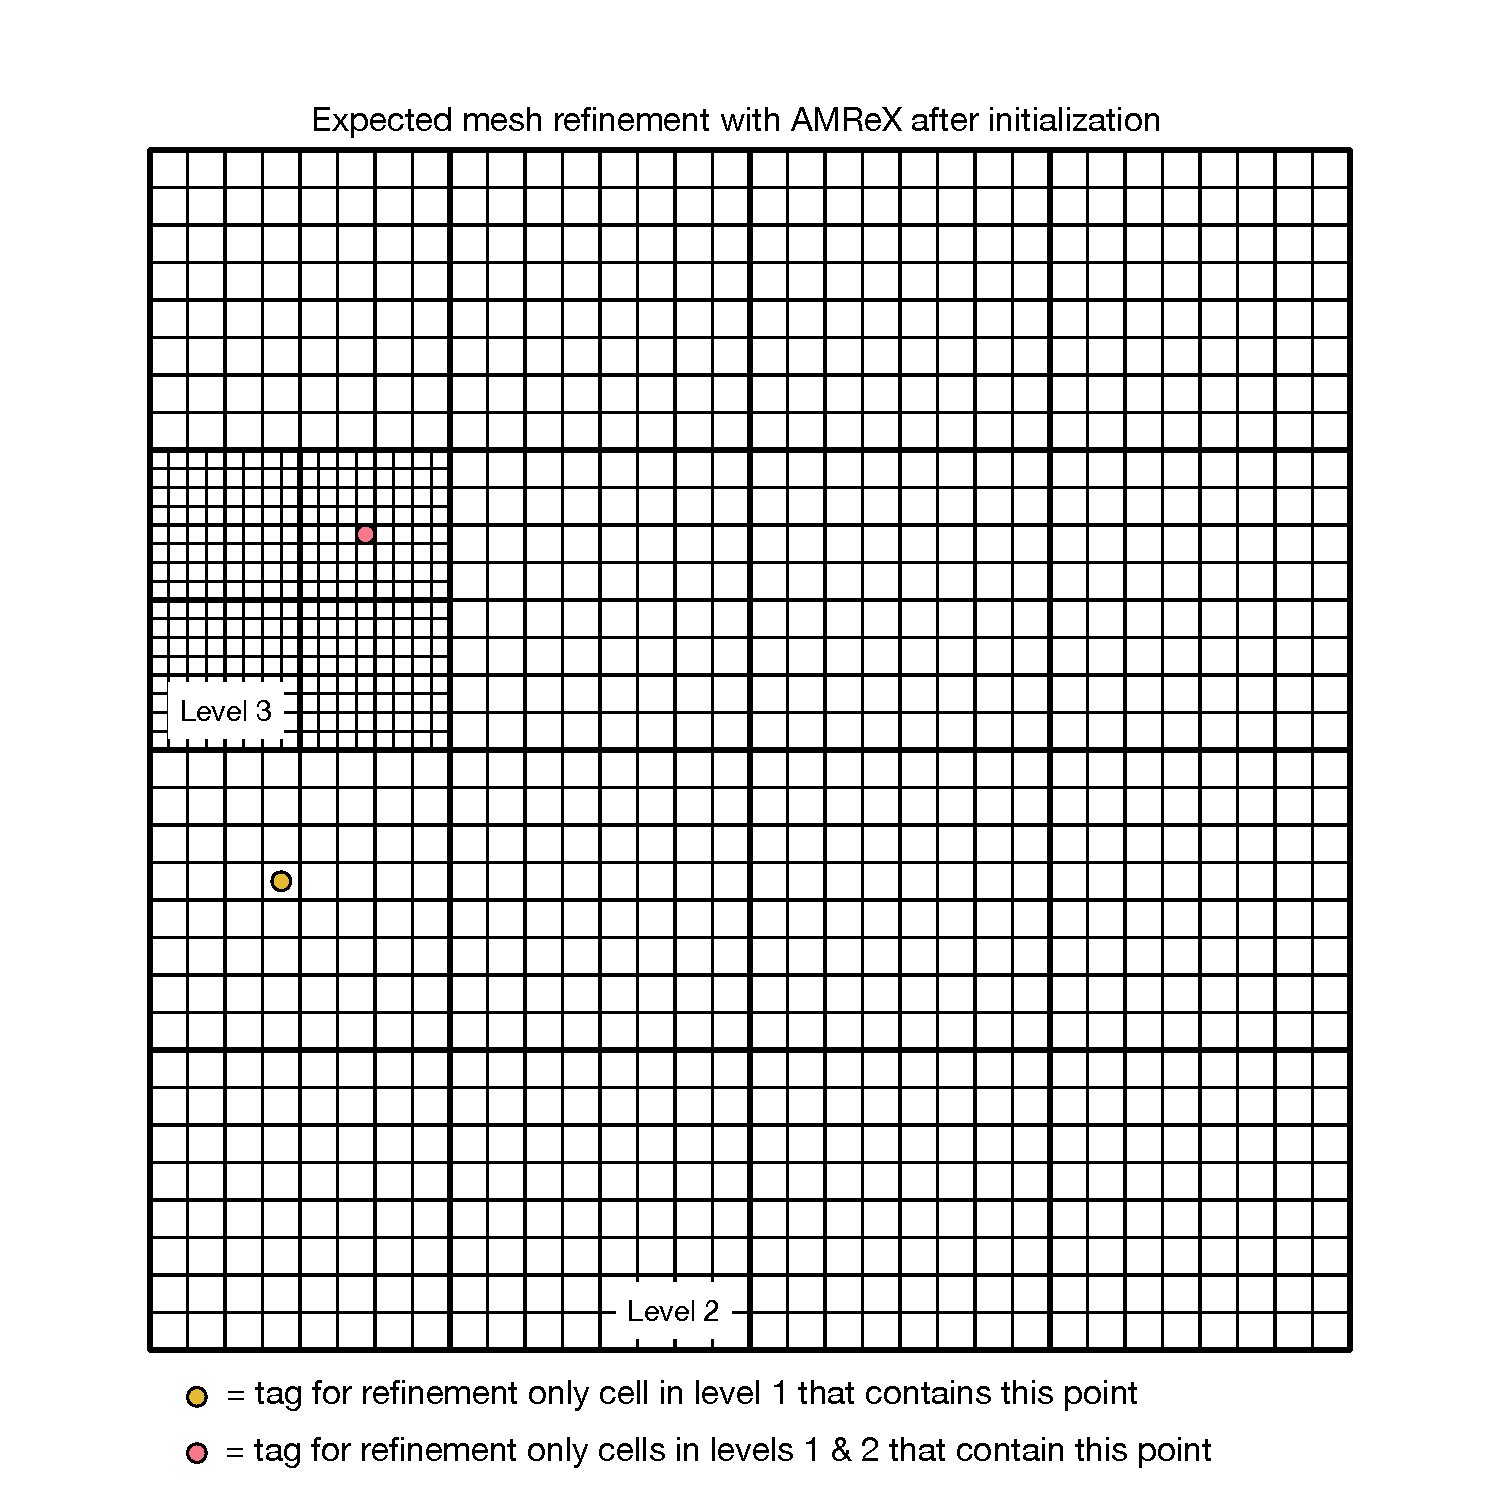
\includegraphics[width=4.25in]{TestRefine_Init_Both.pdf}
\caption{(Init) Refinement of mesh expected with both Paramesh and AMReX after loading
initial conditions and doing initial refinement.  Note that level indexing is
1-based in FLASH.}
\end{center}
\end{figure}

\newpage
\subsection{Steps 1/2}
Expected leaf blocks after initial refinement for both Paramesh and AMReX
\begin{figure}[!hp]
\begin{center}
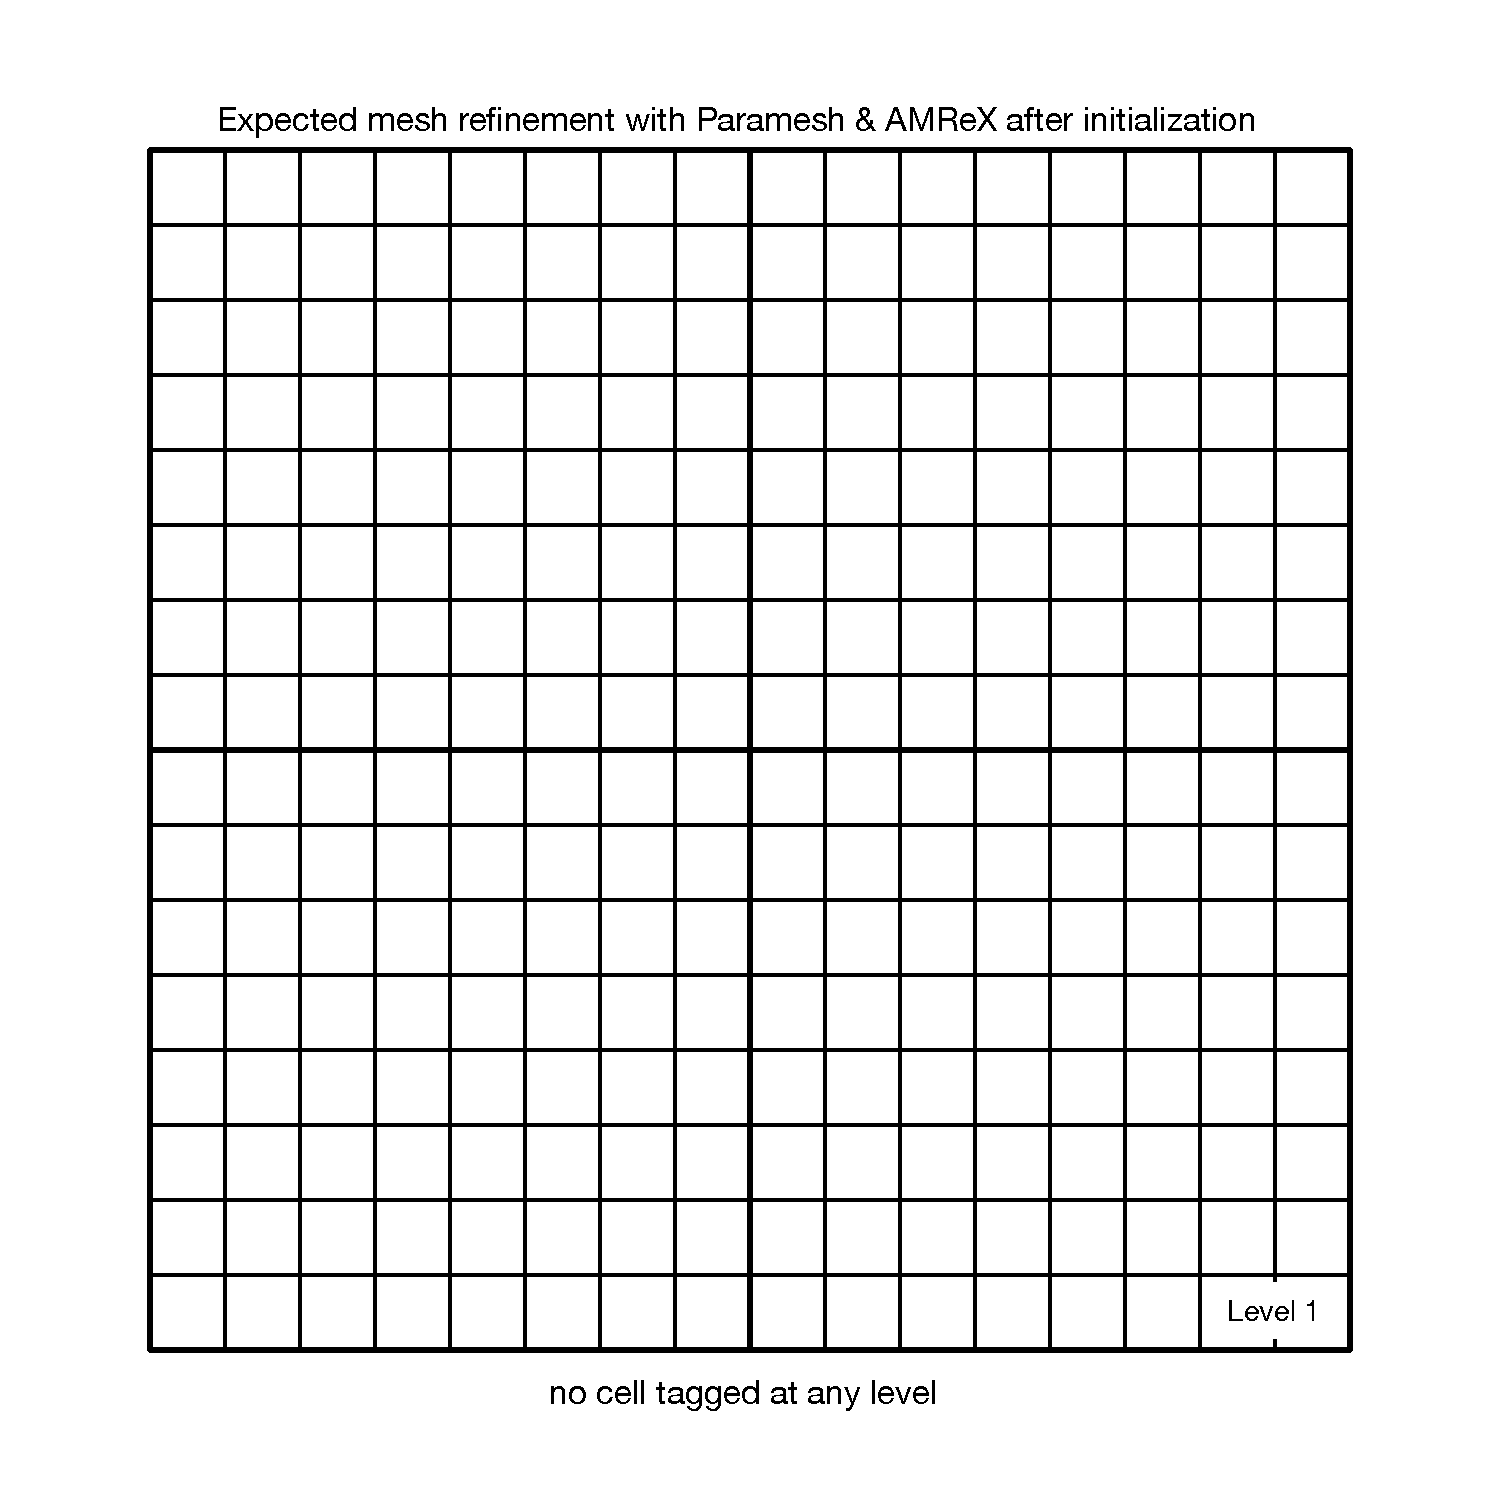
\includegraphics[width=4.25in]{TestRefine_Step2_Both.pdf}\\
\caption{(Step 1) Common refinement expected for Paramesh and achieved with AMReX after
setting all data to zeros at step 1.}
\end{center}
\end{figure}

\newpage
\subsection{Step 3/4}
Expected leaf blocks after step 2 refinement with Paramesh
\begin{figure}[!hp]
\begin{center}
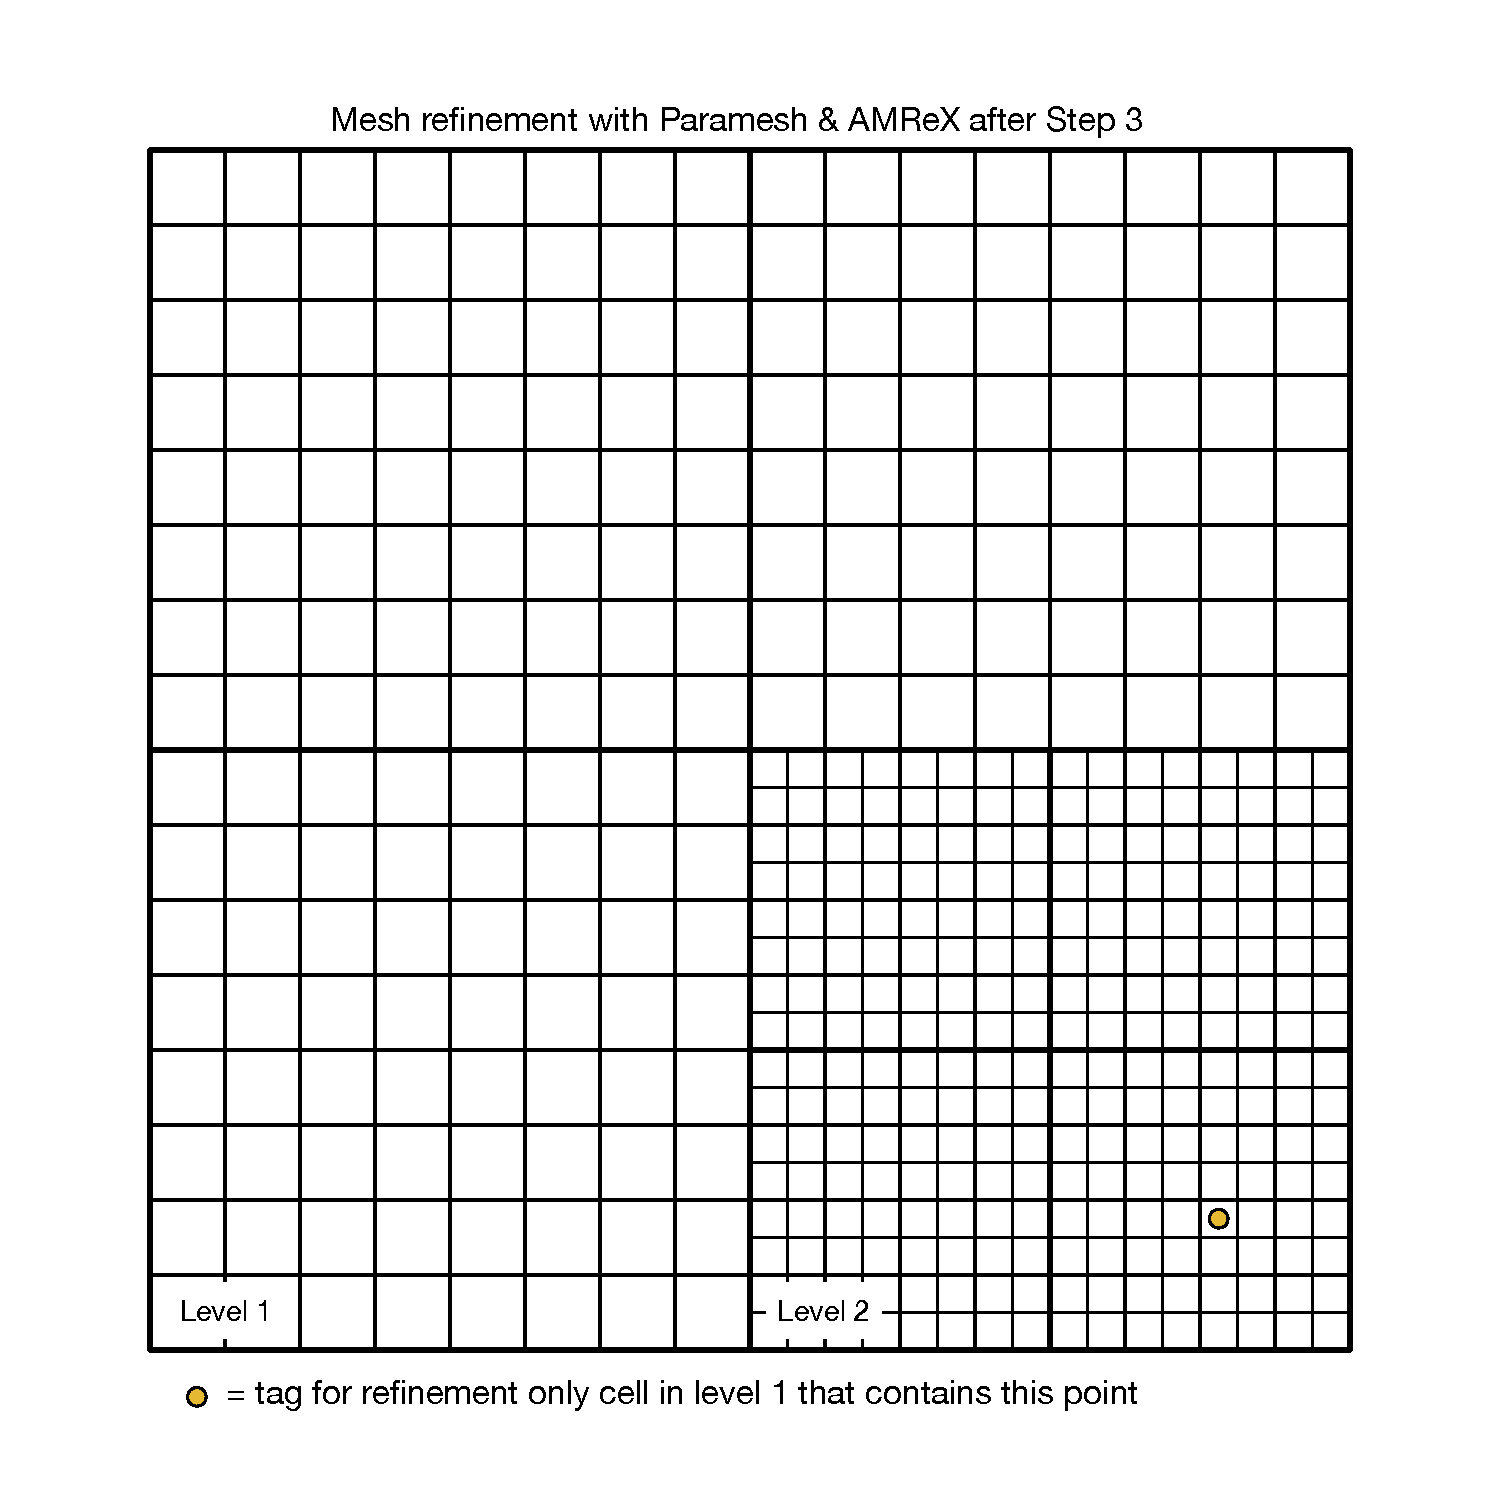
\includegraphics[width=4.25in]{TestRefine_Step4_Both.pdf}
\caption{(Step 3) }
\end{center}
\end{figure}

\newpage
\subsection{Step 5/6}
Leaf blocks achieved after step 8 refinement with AMReX
\begin{figure}[!hp]
\begin{center}
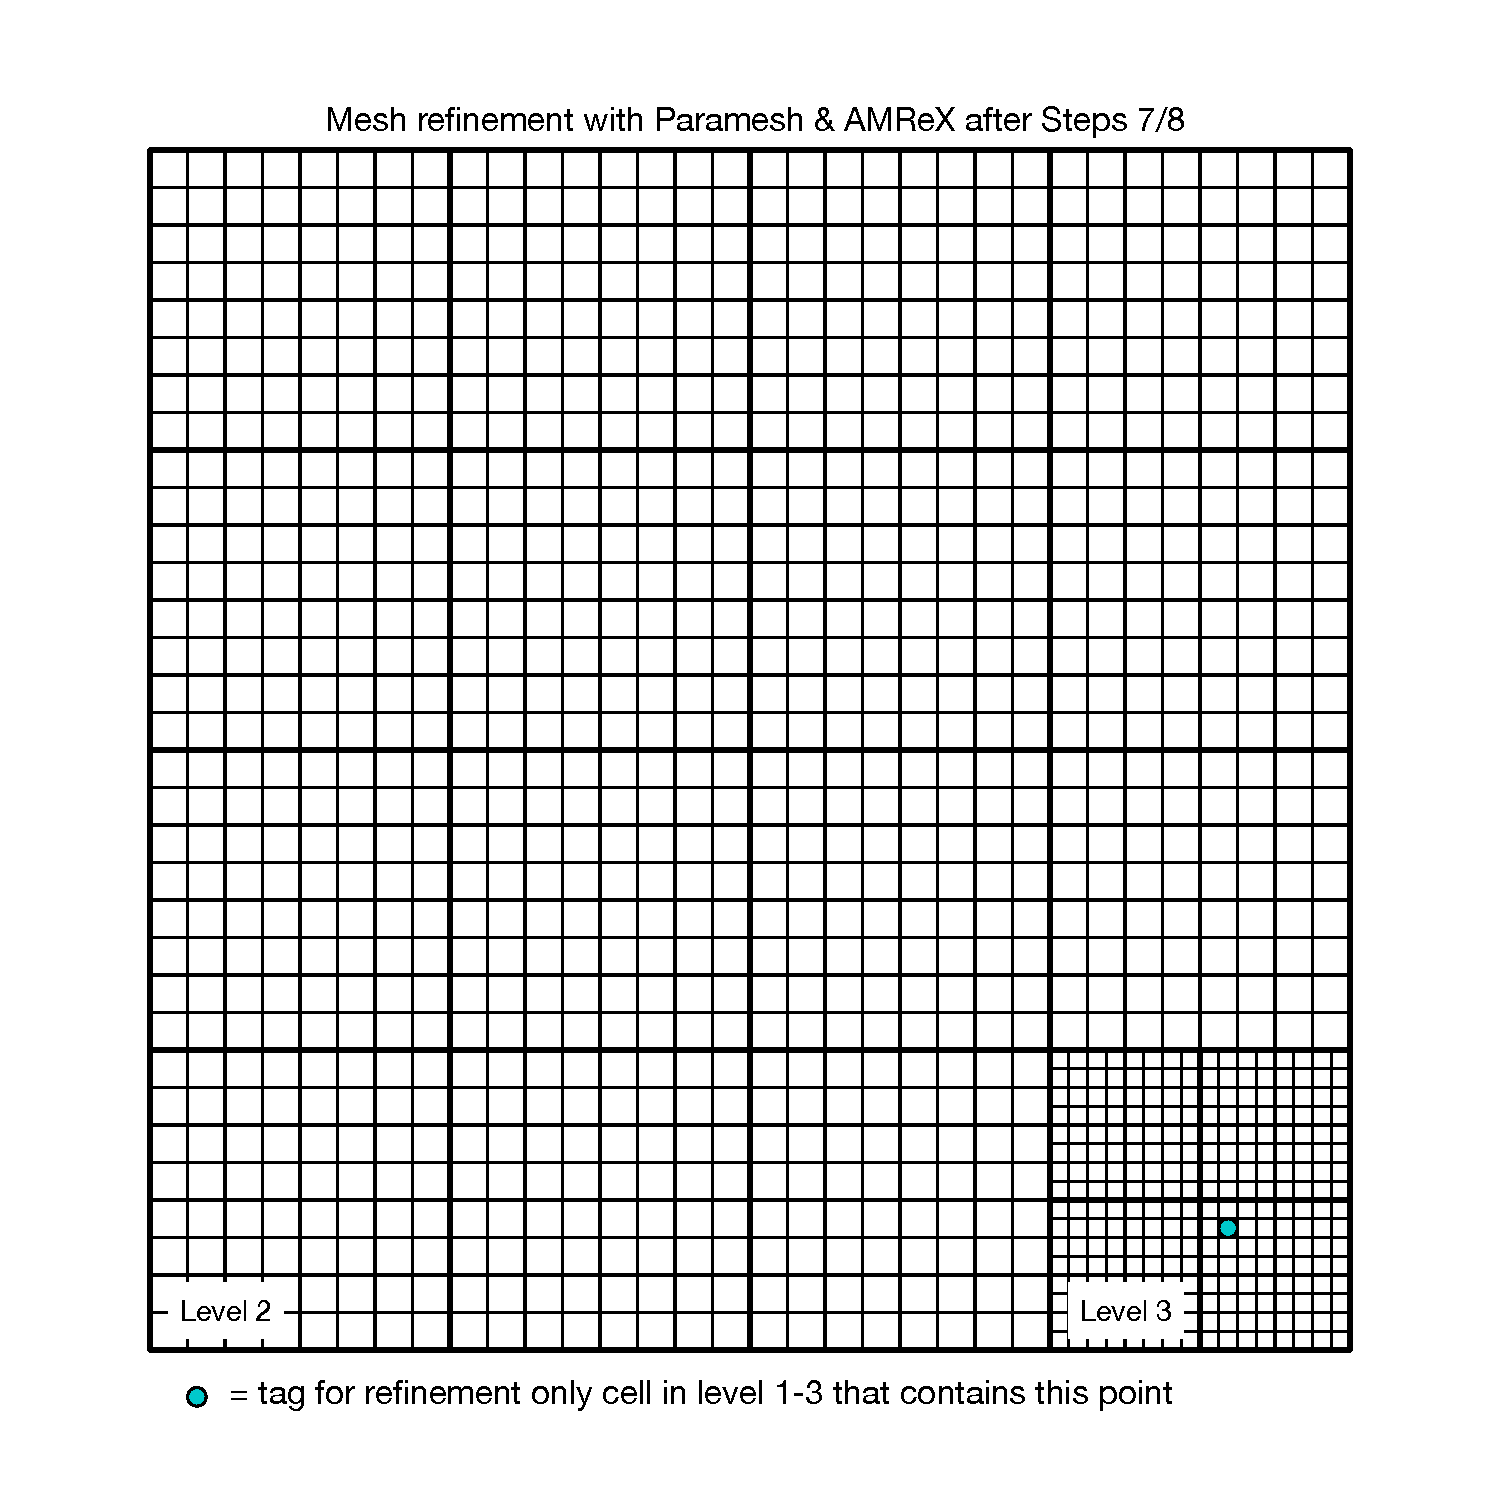
\includegraphics[width=4.25in]{TestRefine_Step6_Both.pdf}
\caption{(Step 4) }
\end{center}
\end{figure}

\newpage
\subsection{Steps 7-10}
Leaf blocks achieved after step 10 refinement with AMReX
\begin{figure}[!hp]
\begin{center}
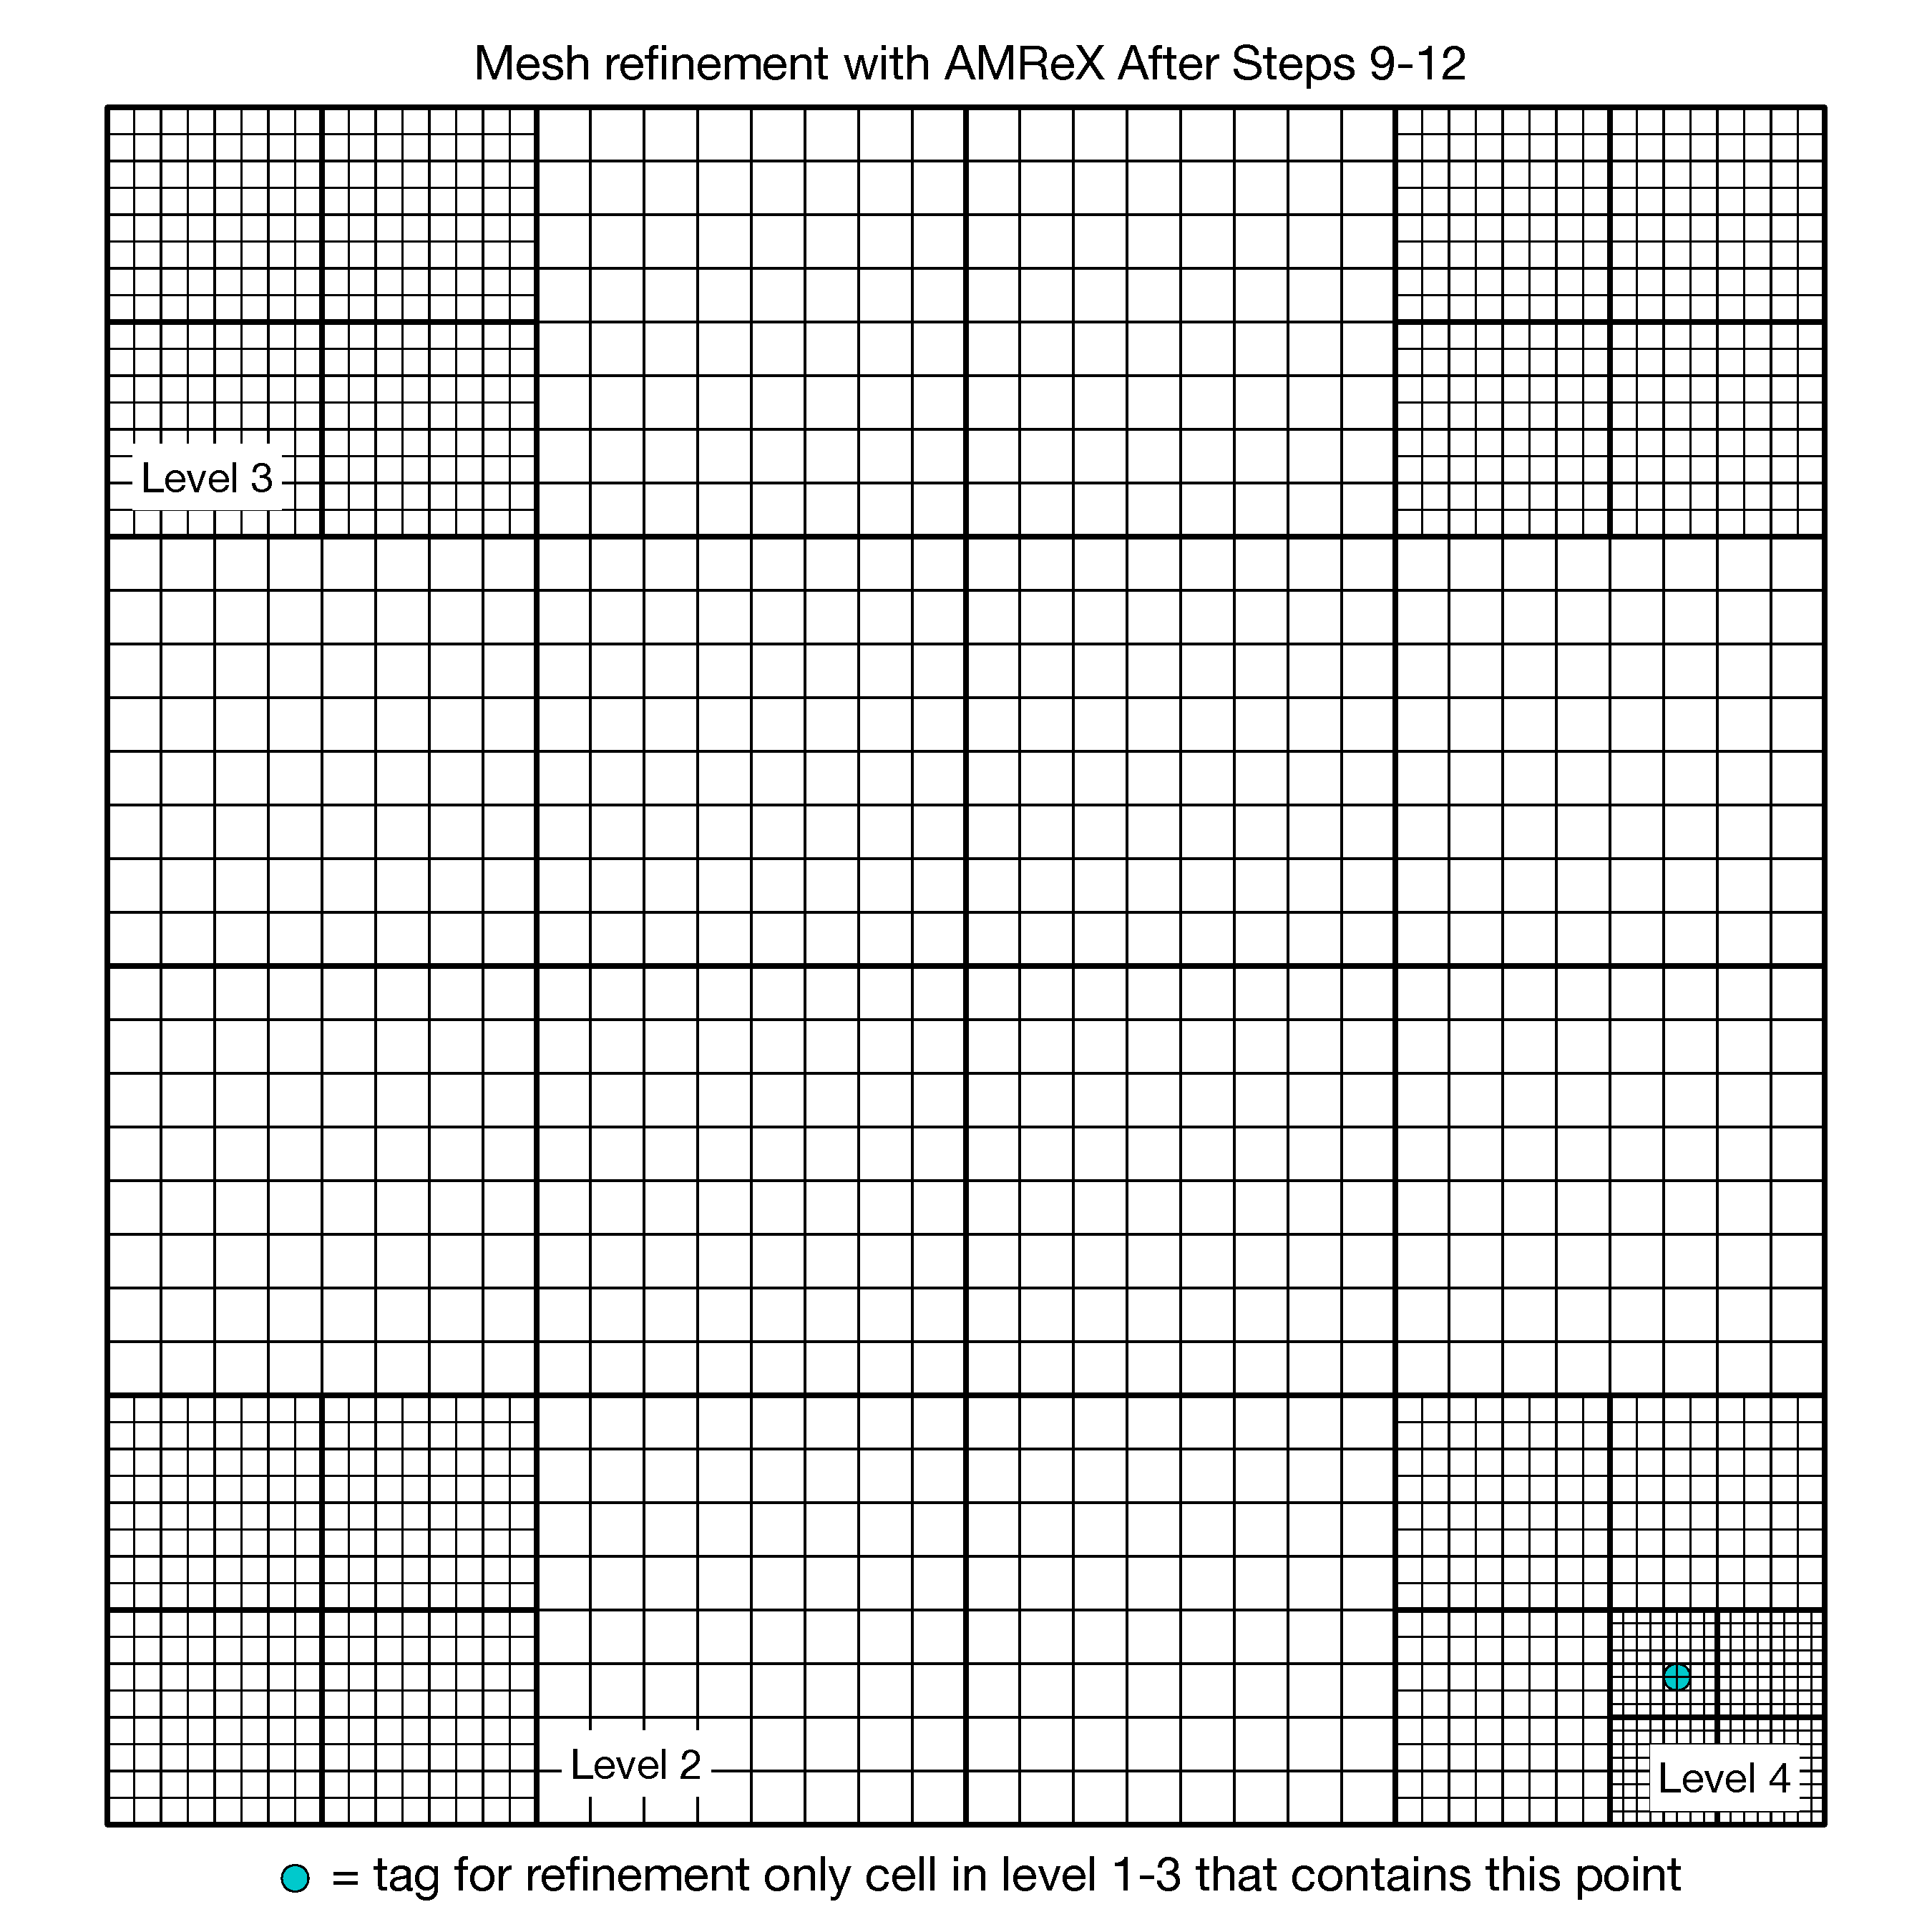
\includegraphics[width=4.25in]{TestRefine_Step8_Both.pdf}
\caption{(Step 5) }
\end{center}
\end{figure}

\newpage
\subsection{Steps 11/12}
Ignore these steps.  They are necessary only to allow the refinement to advance
the new data point to level 3 here.

\subsection{Steps 13/14}
Leaf blocks achieved after step 13 refinement with AMReX
\begin{figure}[!hp]
\begin{center}
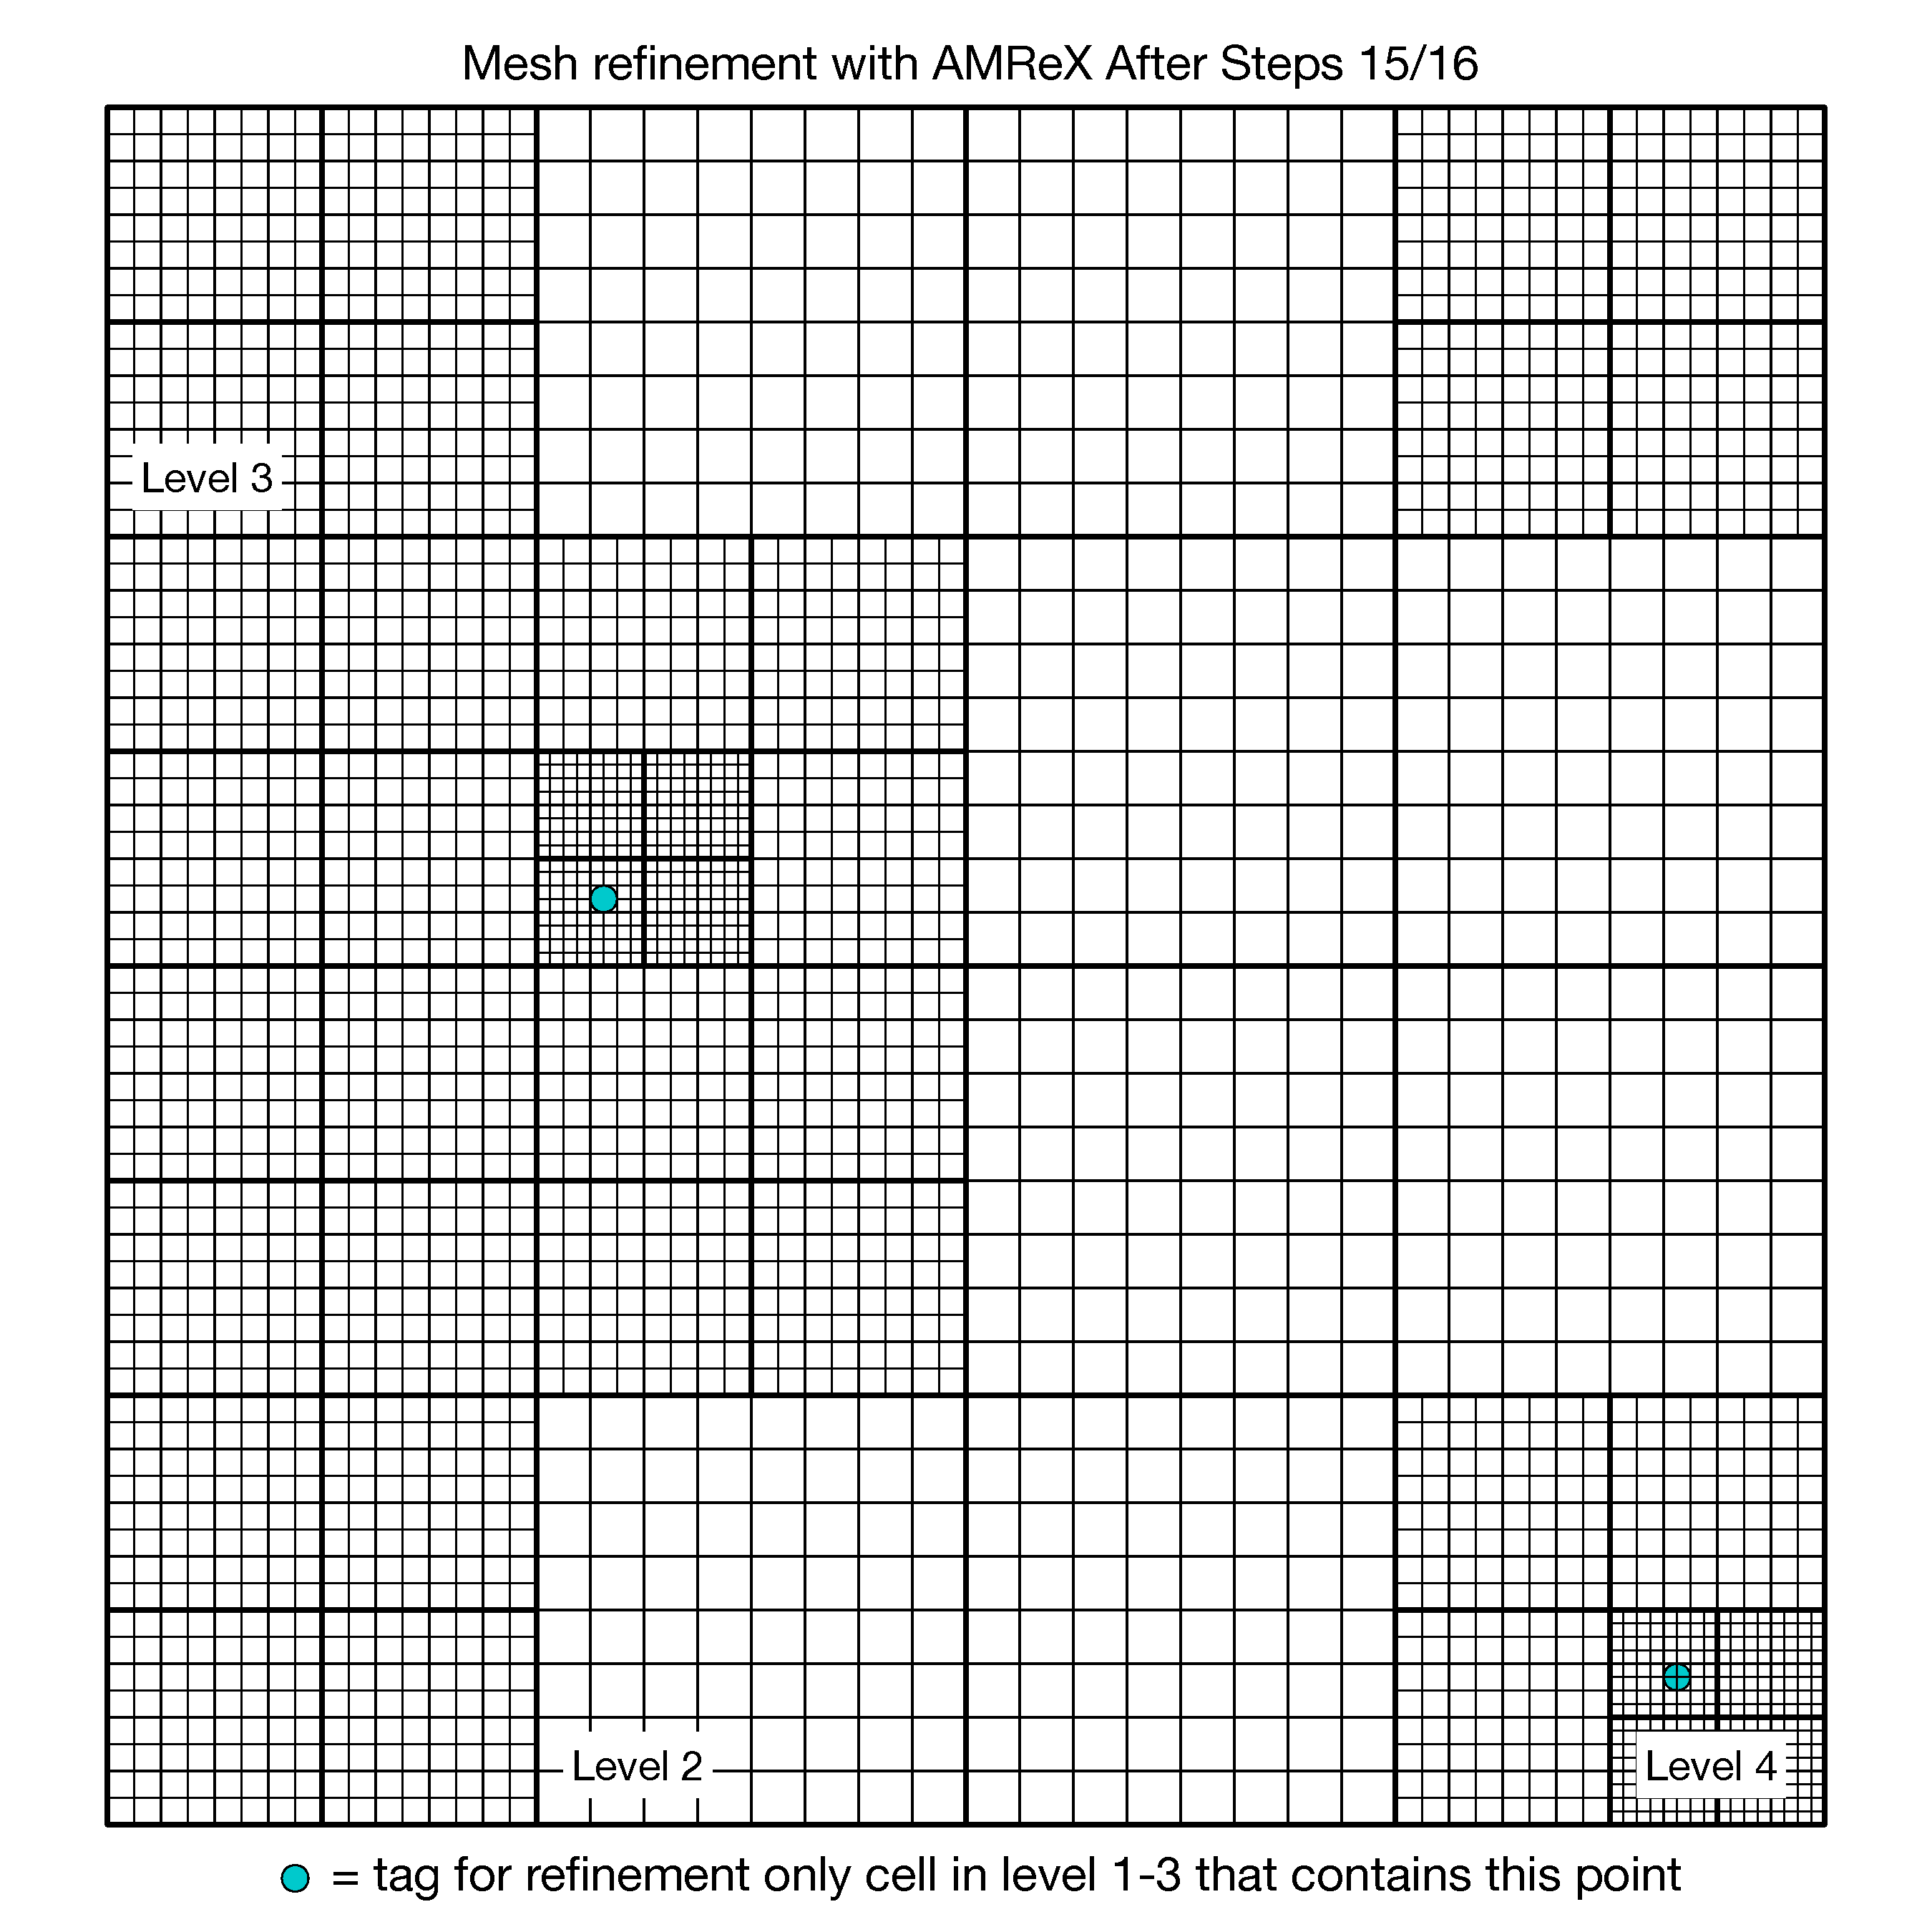
\includegraphics[width=4.25in]{TestRefine_Step14_Both.pdf}
\caption{(Step 6) }
\end{center}
\end{figure}

\newpage
\subsection{Steps 15/16}
All data is zeroed out so that the refinement is reset to a 2x2 block layout on
level 1 as in step 1/2.

\subsection{Steps 16/18}
Correct octree refinement of two blocks independent of which cell is tagged.
This is an example of sacrificing grid efficiency for the organizational
simplicity of octree.  A patch-based scheme might have refined a single block
that is translated to include both of the tag cells.
\begin{figure}[!hp]
\begin{center}
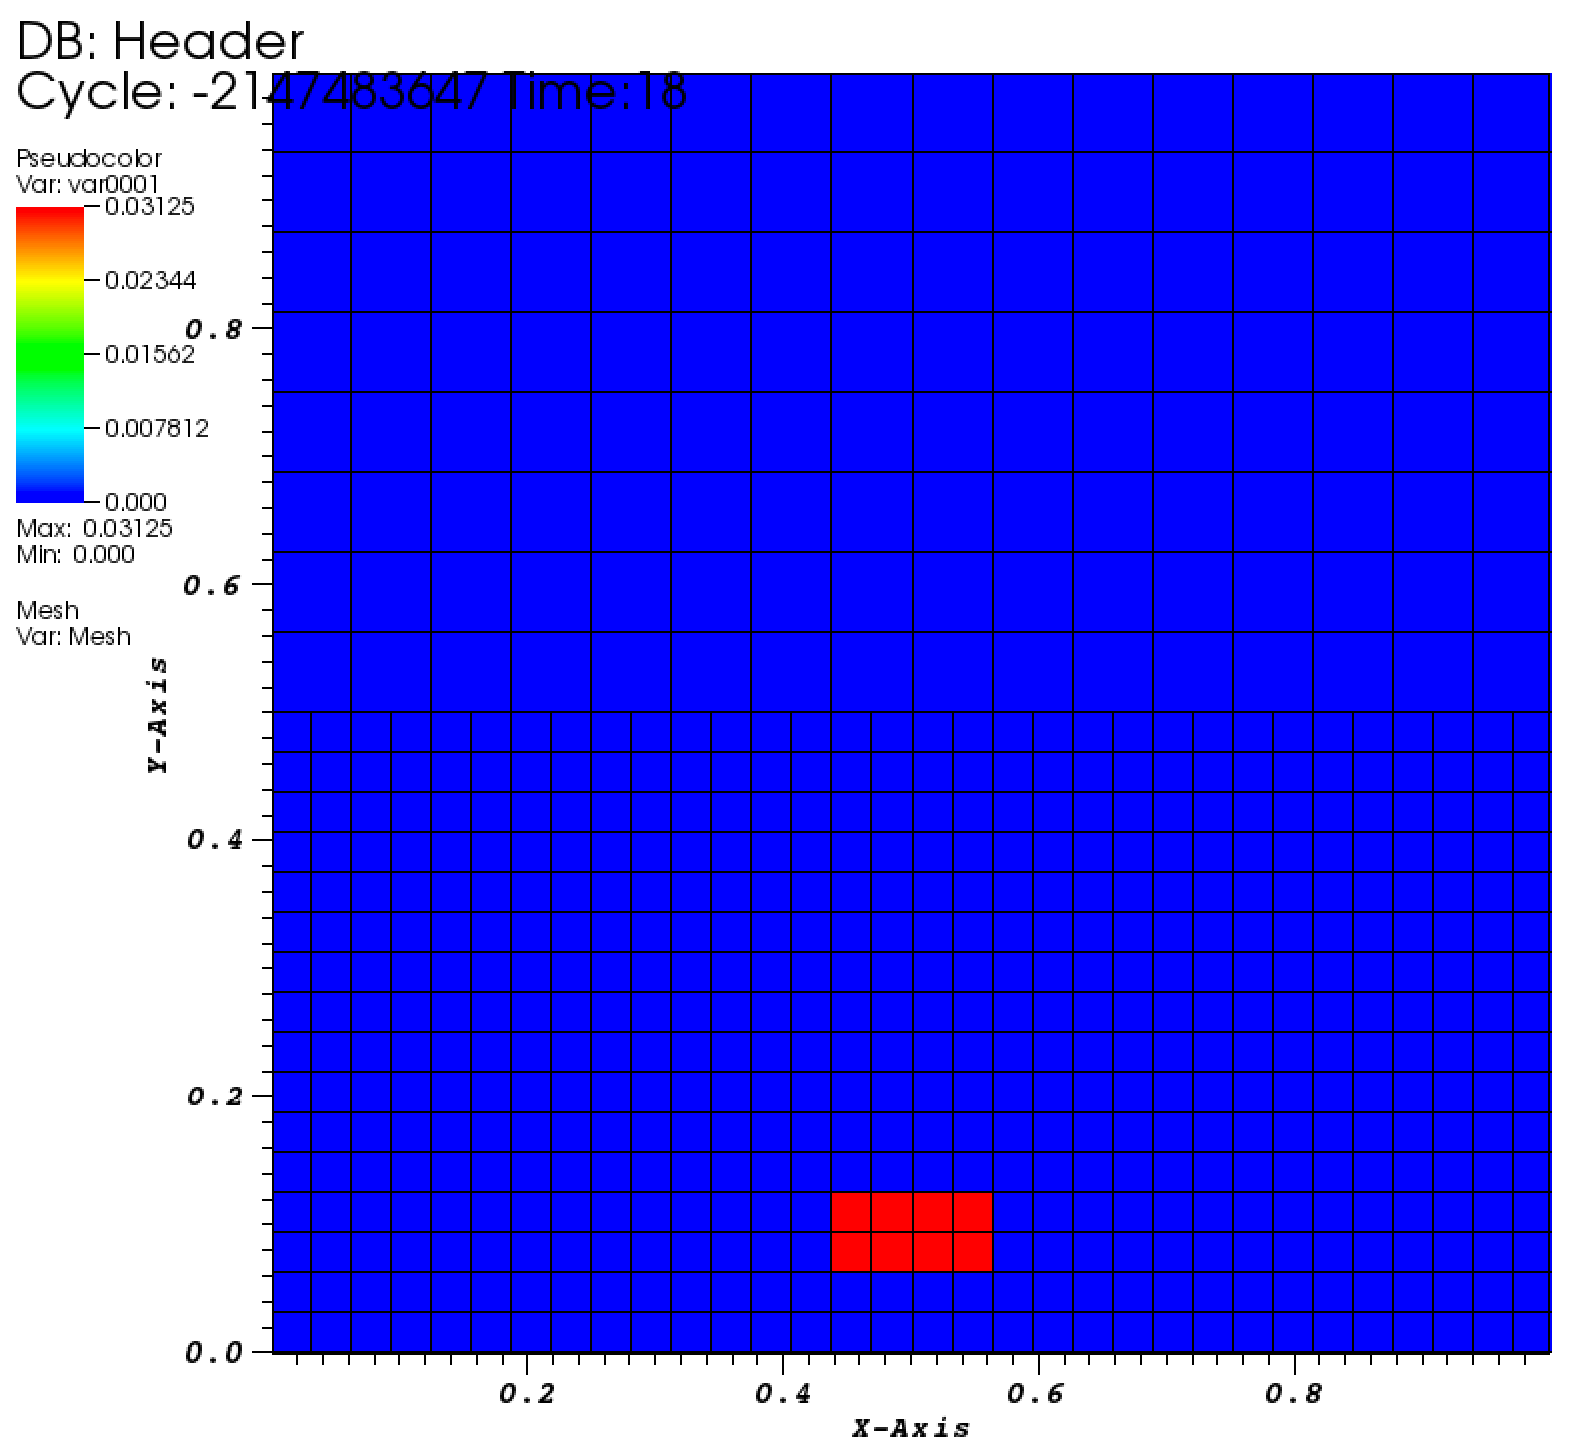
\includegraphics[width=4.25in]{TestRefine_Step18_Both.png}
\caption{(Step 6) }
\end{center}
\end{figure}
\end{document}

